\section{Descriptive Analysis} \label{isect3}
\subsection{Composition of Household Vulnerability Index}
The study uses household characteristics and other information from
the survey, which are more suitable for calculating the household vulnerability of the surveyed households. Table 1 presents various variables used for constructing the households vulnerability index district-wise. Appendix Table 1 presents the VDC-level variables. We define the variables used in our analysis as below:

\begin{singlespace}
	\centering
	\begin{table}[htb]
		\caption{Definition of Variables used for HVI Construction}
		\vspace{0.05cm}
		\renewcommand{\arraystretch}{1.4}
		\resizebox{1.1\textwidth}{!}{%
			\begin{tabular}{p{3cm}p{12cm}} \hline \hline
				Variables & Construct \\ \hline
				hhh\_age & Household head age in years \\
				hhh\_edu & Education attainment of household head \\
				max\_hh\_edu & Highest educational attainment by a household member\\
				implements & Total value of implements such as: Car; Trucks; Motorbike; Plough etc. owned by the household in Rs.\\
				livestock & Total value of livestock (of all types) in Rs.\\
				land & Total area of land owned by the household in sq. m\\
				hh\_caste & Household belonging to the biggest caste in the village (=1) \\
				bank\_saving & Households savings kept in banks or other recognized financial institutions\\
				jewellery & Households' saving in the form of non-productive assets, such as Jewellery. \\
				n\_livelihoods & Count of livelihoods of the households \\ \hline \hline 
			\end{tabular} \\ 		
		}\\ 
		\small{\textit{Source: PEN Dataset}}
	\end{table} 
\end{singlespace}

In the year 2006, the Household Vulnerability Index (HVI) ranged from 0.61 to 0.65 across the survey districts. By 2012, minimal changes were observed, with certain VDCs in the study districts experiencing an improvement. For instance, Chainpur VDC in Chitwan improved its vulnerability position from 0.62 in 2006 to 0.61 in 2009 but remained stagnant at 0.61 in 2012. Similarly, Kunjo VDC in Mustang district reduced its vulnerability from 0.65 in 2006 to 0.64 in 2009, but remained stagnant at 0.64 in 2012. Lete VDC in Mustang district exhibited no change in vulnerability from 2006 to 2009 but saw a decrease from 0.63 in 2006 to 0.62 in 2012. Conversely, Hemja VDC in Kaski district maintained the same vulnerability position over the six-year span. The observed phenomenon of households improving little to not improving its positions aligns with the findings of \cite{acharya2008dimension} that households in rural areas face significant vulnerability.\par 
\begin{landscape}
	\begin{table}
		\vspace{-35pt}
		\caption{ Variables used to construct the Vulnerability Index}
		\renewcommand{\arraystretch}{1.15}
		\resizebox{1.7\textwidth}{!}{%
			\begin{tabular}{lccccccccc} \hline
				\textbf{Year}                    & \multicolumn{3}{c}{\textbf{2006}}                                                                                                                                                                    & \multicolumn{3}{c}{\textbf{2009}}                                                                                                                                                                    & \multicolumn{3}{c}{\textbf{2012}}                                                                                                                                                                    \\ \hline
				\textbf{District}                & \textbf{Chitwan}                                                & \textbf{Kaski}                                                  & \textbf{Mustang}                                                 & \textbf{Chitwan}                                                & \textbf{Kaski}                                                  & \textbf{Mustang}                                                 & \textbf{Chitwan}                                                & \textbf{Kaski}                                                  & \textbf{Mustang}                                                 \\ \hline
				\textbf{Human Capital}           &                                                                 &                                                                 &                                                                  &                                                                 &                                                                 &                                                                  &                                                                 &                                                                 &                                                                  \\ 
				hhh\_age                         & \begin{tabular}[c]{@{}c@{}}50.36 \\ (14.15)\end{tabular}        & \begin{tabular}[c]{@{}c@{}}50.14 \\ (14.57)\end{tabular}        & \begin{tabular}[c]{@{}c@{}}52.89  \\ (13.52)\end{tabular}        & \begin{tabular}[c]{@{}c@{}}52.13  \\ (13.75)\end{tabular}       & \begin{tabular}[c]{@{}c@{}}52.00  \\ (13.39)\end{tabular}       & \begin{tabular}[c]{@{}c@{}}54.12  \\ (13.78)\end{tabular}        & \begin{tabular}[c]{@{}c@{}}52.24  \\ (17.20)\end{tabular}       & \begin{tabular}[c]{@{}c@{}}53.52  \\ (13.71)\end{tabular}       & \begin{tabular}[c]{@{}c@{}}55.24  \\ (14.17)\end{tabular}        \\
				hhh\_edu                         & \begin{tabular}[c]{@{}c@{}}3.08  \\ (4.06)\end{tabular}         & \begin{tabular}[c]{@{}c@{}}6.29  \\ (4.97)\end{tabular}         & \begin{tabular}[c]{@{}c@{}}3.05  \\ (3.98)\end{tabular}          & \begin{tabular}[c]{@{}c@{}}2.93  \\ (4.06)\end{tabular}         & \begin{tabular}[c]{@{}c@{}}6.07  \\ (5.23)\end{tabular}         & \begin{tabular}[c]{@{}c@{}}2.94  \\ (3.78)\end{tabular}          & \begin{tabular}[c]{@{}c@{}}2.91  \\ (4.33)\end{tabular}         & \begin{tabular}[c]{@{}c@{}}6.91  \\ (5.07)\end{tabular}         & \begin{tabular}[c]{@{}c@{}}2.90  \\ (4.08)\end{tabular}          \\
				max\_hh\_edu                     & \begin{tabular}[c]{@{}c@{}}8.44  \\ (3.91)\end{tabular}         & \begin{tabular}[c]{@{}c@{}}10.76  \\ (2.90)\end{tabular}        & \begin{tabular}[c]{@{}c@{}}7.64  \\ (3.32)\end{tabular}          & \begin{tabular}[c]{@{}c@{}}9.70  \\ (3.63)\end{tabular}         & \begin{tabular}[c]{@{}c@{}}11.18  \\ (3.94)\end{tabular}        & \begin{tabular}[c]{@{}c@{}}8.04  \\ (3.93)\end{tabular}          & \begin{tabular}[c]{@{}c@{}}9.89  \\ (4.44)\end{tabular}         & \begin{tabular}[c]{@{}c@{}}11.91 \\  (4.03)\end{tabular}        & \begin{tabular}[c]{@{}c@{}}8.22  \\ (3.87)\end{tabular}          \\
				\textbf{Physical Capital}        &                                                                 &                                                                 &                                                                  &                                                                 &                                                                 &                                                                  &                                                                 &                                                                 &                                                                  \\
				implements                       & \begin{tabular}[c]{@{}c@{}}4660.32  \\ (11275.51)\end{tabular}  & \begin{tabular}[c]{@{}c@{}}14057.03  \\ (16860.40)\end{tabular} & \begin{tabular}[c]{@{}c@{}}10360.32  \\ (19629.35)\end{tabular}  & \begin{tabular}[c]{@{}c@{}}10153.80  \\ (23970.96)\end{tabular} & \begin{tabular}[c]{@{}c@{}}30700.04  \\ (46128.42)\end{tabular} & \begin{tabular}[c]{@{}c@{}}15135.16  \\ (25508.99)\end{tabular}  & \begin{tabular}[c]{@{}c@{}}22165.29  \\ (38089.26)\end{tabular} & \begin{tabular}[c]{@{}c@{}}48959.03  \\ (70582.61)\end{tabular} & \begin{tabular}[c]{@{}c@{}}21466.58  \\ (27566.06)\end{tabular}  \\
				livestock                        & \begin{tabular}[c]{@{}c@{}}18532.68  \\ (15428.31)\end{tabular} & \begin{tabular}[c]{@{}c@{}}26573.08  \\ (20411.58)\end{tabular} & \begin{tabular}[c]{@{}c@{}}80387.77  \\ (224589.10)\end{tabular} & \begin{tabular}[c]{@{}c@{}}43936.83  \\ (39679.86)\end{tabular} & \begin{tabular}[c]{@{}c@{}}35690.11  \\ (35760.04)\end{tabular} & \begin{tabular}[c]{@{}c@{}}56165.26  \\ (178639.73)\end{tabular} & \begin{tabular}[c]{@{}c@{}}38993.71  \\ (34330.39)\end{tabular} & \begin{tabular}[c]{@{}c@{}}34635.85  \\ (39306.64)\end{tabular} & \begin{tabular}[c]{@{}c@{}}34114.52  \\ (39335.73)\end{tabular}  \\
				land                             & \begin{tabular}[c]{@{}c@{}}2027.47  \\ (6367.27)\end{tabular}   & \begin{tabular}[c]{@{}c@{}}1187.00  \\ (1013.02)\end{tabular}   & \begin{tabular}[c]{@{}c@{}}2940.39  \\ (2789.36)\end{tabular}    & \begin{tabular}[c]{@{}c@{}}915.91  \\ (765.38)\end{tabular}     & \begin{tabular}[c]{@{}c@{}}1491.41  \\ (2060.26)\end{tabular}   & \begin{tabular}[c]{@{}c@{}}2235.09  \\ (3738.40)\end{tabular}    & \begin{tabular}[c]{@{}c@{}}1041.46  \\ (1136.88)\end{tabular}   & \begin{tabular}[c]{@{}c@{}}1374.96  \\ (2253.95)\end{tabular}   & \begin{tabular}[c]{@{}c@{}}1921.22  \\ (1892.77)\end{tabular}    \\
				\textbf{Social Capital}          &                                                                 &                                                                 &                                                                  &                                                                 &                                                                 &                                                                  &                                                                 &                                                                 &                                                                  \\
				hh\_caste                        & \begin{tabular}[c]{@{}c@{}}0.58  \\ (0.50)\end{tabular}         & \begin{tabular}[c]{@{}c@{}}0.89  \\ (0.32)\end{tabular}         & \begin{tabular}[c]{@{}c@{}}0.49  \\ (0.50)\end{tabular}          & \begin{tabular}[c]{@{}c@{}}0.66  \\ (0.48)\end{tabular}         & \begin{tabular}[c]{@{}c@{}}0.98  \\ (0.14)\end{tabular}         & \begin{tabular}[c]{@{}c@{}}0.58  \\ (0.50)\end{tabular}          & \begin{tabular}[c]{@{}c@{}}0.50  \\ (0.50)\end{tabular}         & \begin{tabular}[c]{@{}c@{}}0.86  \\ (0.50)\end{tabular}         & \begin{tabular}[c]{@{}c@{}}0.59 \\ (0.42)\end{tabular}           \\
				\textbf{Financial Capital}       &                                                                 &                                                                 &                                                                  &                                                                 &                                                                 &                                                                  &                                                                 &                                                                 &                                                                  \\
				bank\_saving                     & \begin{tabular}[c]{@{}c@{}}879.58  \\ (2661.50)\end{tabular}    & \begin{tabular}[c]{@{}c@{}}9663.83  \\ (26812.59)\end{tabular}  & \begin{tabular}[c]{@{}c@{}}31897.65  \\ (79933.66 )\end{tabular} & \begin{tabular}[c]{@{}c@{}}1911.63  \\ (6126.69)\end{tabular}   & \begin{tabular}[c]{@{}c@{}}11937.72  \\ (31025.90)\end{tabular} & \begin{tabular}[c]{@{}c@{}}24536.06  \\ (59338.85)\end{tabular}  & \begin{tabular}[c]{@{}c@{}}11953.55  \\ (31763.88)\end{tabular} & \begin{tabular}[c]{@{}c@{}}25410.64  \\ (66932.36)\end{tabular} & \begin{tabular}[c]{@{}c@{}}48051.24  \\ (104495.00)\end{tabular} \\
				jewellery                        & \begin{tabular}[c]{@{}c@{}}0.00  \\ (0.00)\end{tabular}         & \begin{tabular}[c]{@{}c@{}}0.00  \\ (0.00)\end{tabular}         & \begin{tabular}[c]{@{}c@{}}31662.91  \\ (67846.57)\end{tabular}  & \begin{tabular}[c]{@{}c@{}}4396.88  \\ (6965.54)\end{tabular}   & \begin{tabular}[c]{@{}c@{}}20485.87  \\ (16594.27)\end{tabular} & \begin{tabular}[c]{@{}c@{}}38598.35  \\ (79440.96)\end{tabular}  & \begin{tabular}[c]{@{}c@{}}21477.20  \\ (23620.48)\end{tabular} & \begin{tabular}[c]{@{}c@{}}51605.95  \\ (48463.66)\end{tabular} & \begin{tabular}[c]{@{}c@{}}54132.35  \\ (112328.06)\end{tabular} \\
				\textbf{Livelihood}              &                                                                 &                                                                 &                                                                  &                                                                 &                                                                 &                                                                  &                                                                 &                                                                 &                                                                  \\
				n\_livelihoods                   & \begin{tabular}[c]{@{}c@{}}4.81\\ (0.97)\end{tabular}           & \begin{tabular}[c]{@{}c@{}}4.72\\ (0.91)\end{tabular}           & \begin{tabular}[c]{@{}c@{}}4.56\\ (0.93)\end{tabular}            & \begin{tabular}[c]{@{}c@{}}4.93\\ (1.02)\end{tabular}           & \begin{tabular}[c]{@{}c@{}}4.74\\ (0.91)\end{tabular}           & \begin{tabular}[c]{@{}c@{}}5.11\\ (0.84)\end{tabular}            & \begin{tabular}[c]{@{}c@{}}4.60\\ (0.98)\end{tabular}           & \begin{tabular}[c]{@{}c@{}}4.78\\ (0.90)\end{tabular}           & \begin{tabular}[c]{@{}c@{}}4.60\\ (0.98)\end{tabular}            \\
				\textbf{Household Vulnerability} &                                                                 &                                                                 &                                                                  &                                                                 &                                                                 &                                                                  &                                                                 &                                                                 &                                                                  \\
				HVI                              & \begin{tabular}[c]{@{}c@{}}0.61  \\ (0.05)\end{tabular}         & \begin{tabular}[c]{@{}c@{}}0.62  \\ (0.04)\end{tabular}         & \begin{tabular}[c]{@{}c@{}}0.64  \\ (0.05)\end{tabular}          & \begin{tabular}[c]{@{}c@{}}0.61  \\ (0.05)\end{tabular}         & \begin{tabular}[c]{@{}c@{}}0.62  \\ (0.04)\end{tabular}         & \begin{tabular}[c]{@{}c@{}}0.63  \\ (0.05)\end{tabular}          & \begin{tabular}[c]{@{}c@{}}0.61  \\ (0.05)\end{tabular}         & \begin{tabular}[c]{@{}c@{}}0.62  \\ (0.05)\end{tabular}         & \begin{tabular}[c]{@{}c@{}}0.63  \\ (0.05)\end{tabular}         \\ \hline \hline
			\end{tabular}
		}
		\small{\textit{Note:SD in the parenthesis\\ [-0.9ex]
				Source: Author's Calculation}}
			\label{tab:hvivariables}
	\end{table}
\end{landscape}
	
\subsubsection{Human Capital}	
Household Head Age, Education and Maximum educational attainment by the household member were taken as the Human Capital of the households. Household head age as a measure of experience and knowledge has been taken as a contributing factor in Human Capital of the households. The average age of the household head was 52 years in 2006, 53 in year 2009 and 54 in year 2012 (see table \ref{tab:hvivariables}). This progression in the household head age positively affects human capital.\par 

On household head education, Hemja VDC of Kaski district has made a jump of 6 to 7 mean years of schooling from 2006 to 2012. Similarly, Lete VDC of Mustang district has made a negligible progress of 3.25 to 3.3 mean years of schooling. Chainpur VDC of Chitwan district and Kunjo VDC of Mustang district has made negative progress. This mixed progression of household head educational attainment will have mixed effect on human capital.\par  

All VDCs have made positive improvement in part of maximum educational attainment by the household members. Hemja VDC has the highest mean years of schooling of the household members. It has made a remarkable progress from 10 mean years of schooling to 12 from 2006 to 2012. Chainpur VDC also has followed the similar trajectory. It had mean of 8 years of schooling in 2006 and it improved to 10 by the end of 2012. Lete VDC had 8.14 mean years of schooling in the year 2006 which only slightly improved to 8.7 in the year 2012. Kunjo VDC has the least mean years of educational attainment by the household member with 7.1 years in 2006 to 7.72 in 2012. The improvement in the schooling years would affect the human capital positively.\par 

\subsubsection{Physical Capital}
Chainpur VDC had the least implements in the year 2006 whereas Hemja had the highest level of implements in the same year. But, chainpur made remarkable progress by increasing its implements by 118\%  by the end of 2009 and exactly the same increase by the end of the year 2012. Hemja also experience the same rate of growth of implements in the year 2009 but the rate declined to 59\% in the year 2012. Kunjo and Lete, both VDC of Mustang could improve its implements position in the year 2009 by 77\% and 32\% respectively. However, both VDC had a decline in the growth of the implements in the last wave of the survey. Kunjo's increase of the implements was 69\% and Lete's was only 25\% (see table \ref{tab:hvivariables}).\par  

In part of Livestock holdings, Lete VDC had the highest holding in the year 2006 whereas Chainpur had the least holding of the livestock. However, Chainpur managed to increase its livestock-holding by 137\% at the end of year 2009. But Chainpur VDC's livestock holding declined by 11\% by the end of 2012. Kunjo was the second place after Lete in the livestock holding in year 2006. But, its livestock-holding declined continuously in the following years 2009 and 2012 by 25\% and 11\% respectively. Lete VDC despite holding the most livestock in the year 2006 had a severe decline in its livestock holding placing itself as the least livestock-holding VDC by the end of year 2012. It experienced the decrease of 33\% in the year 2009 and almost 60\% in the year 2012.\par  

Lete VDC had the highest land holding followed by Kunjo VDC in the year 2006. Kaski had the least land holdings in the same year. Chainpur then followed Kaski. In year 2009, Chainpur had a decline of 55\% whereas Kunjo and Lete had a decline of 14\% and 33\% respectively. Hemja, however, increased its land-holding by 26\% by the end of 2009. Chainpur, despite experiencing decrease in land-holding, managed to increase the land-holding by 14\% by the end of 2012. In the same period, all 3 VDCs': Hemja; Kunjo; and Lete experienced decline in the land-holding by 8\%, 13\% and 15\% respectively.\par 

\subsubsection{Social Capital}  
Following \cite{alha2018other, vanneman2006social}, the caste was considered as a social capital. Belonging to the largest caste improves the household's network within the community as well as across the community. Thus it helps the households to negate the effects of uncertain events. So, belonging to largest caste have a negative influence on the household vulnerability. In the year 2006 Hemja had the highest percentage of Household head i.e. 89\% belonging to largest caste. Whereas Kunjo had the least percentage of the household heads belonging to the largest caste in the village. The trend followed with increase in the percentage of the household heads belonging to the largest caste in the year 2009. Chainpur, Hemja, Kunjo and Lete had the percentage change of household heads belonging to largest caste increase by 13\%, 10\%, 19\% and 17\% respectively(see table \ref{tab:hvivariables}).\par  

However, the percentage change declined by 23\% and 48\% for Chainpur and Hemja respectively in the year 2012. Kunjo and Lete, however experience an increase of the percentage of household heads belonging to caste by 65\% and 8\% in the year 2012 respectively.\par 

\subsubsection{Financial Capital}
Bank savings and Jewellery are considered as the financial capitals. The financial capital play a huge part in the welfare of the households.\par 

Lete VDC had the highest bank savings in the year 2006 and the trend continued until the final wave of the survey year 2012. It experienced decline of the saving in the year 2009 relative to 2006 by 11\% but it managed to increase its saving by 114\% by the end of 2012. Chainpur had a opposite experience than that of Lete. It had the least bank saving among all VDCs in the year 2006 and it persisted to have least of it in the final wave of the survey year 2012. However, it managed to increase its own saving by 117\% in the year 2009 and 525\% by the end of 2012.\par 

Kunjo had a fairly fluctuating trend with respect to bank saving. It followed Lete to have the second highest possession of bank saving in the year 2006. Though it managed to maintain the position in terms of ranking it had a decline of 41\% in the second of wave of survey year 2009. In the following wave of the survey it experienced an increase of savings by 54\%. But, it fell below the previous ranking. Hemja had a moderate growth of its saving in the year 2009 of 24\%. The rate leaped to 113\% by the end of 2012 (see table \ref{tab:hvivariables}).\par     

The data for jewellery possession were not available for Chainpur and Hemja VDC for the year 2006. So comparing between Kunjo and Lete, Lete had the highest possession of jewellery. It continued to have the highest jewellery possession in the following wave of surveys. The rate of increase remained moderate of 13\% and 22\% in the year 2009 and 2012 respectively. Kunjo, on the other hand, have aggressively increased its jewellery possession by 45\% in the year 2009 and 80\% in the year 2012.\par 

Data for jewellery possession were available for Chainpur and Hemja for 2009 and 2012. Chainpur had the least possession in the year 2009. But, it managed to increased its possession by 388\% in the year 2012 which is the highest rate of increase among all VDCs. Nonetheless, it persisted in the VDC having the least possession of jewellery in the final wave of survey year 2012.\par

\subsubsection{Livelihood Options}
This includes the diversity of livelihood options that the households in the particular area in the particular period of time. The livelihood is considered a capital because having diversified income can raise household income, reduce risk, and improve their livelihoods \citep{scoones2013livelihoods}. All of the VDCs have a relatively similar livelihood counts. In the year 2006, the number of livelihood strategies that the households adopted ranged from 4.32 to 4.81. Kunjo had the least number of livelihood strategies while Chainpur had a relatively more number of strategies. The average number of livelihood strategies have increased in the year 2009. But, the rate of increase is fairly mild for Chainpur with only 2\% increase and Hemja with only 0.4\%.  As for Kunjo, it had an increase of 11\% in their livelihood counts. Lete had an increase of 12\% in the year 2009. In the year 2012, all VDCs except for Hemja experienced downward sloping livelihood counts. Hemja observed a growth of 0.84\% in livelihood strategies, while Chainpur, Kunjo, and Lete exhibited reduced growth rates of 7\%, 11\%, and 8\%, respectively (see table \ref{tab:hvivariables}).

\subsection{Environmental Dependence and Household Vulnerability}
Table 2 presents the factors that are likely to affect Household vulnerability with central emphasis on Environmental dependence. The table consists of four critical variables which are assumed to affect the household vulnerability. The definition of the variables are in Table 3.2. The variables are: Environmental dependence; Dependency ratio; and Shock.


\begin{table}[htb]
	\caption{Household Vulnerability and Environmental Dependence}
	\renewcommand{\arraystretch}{0.9}
	\resizebox{1\linewidth}{!}{
		\begin{center}
			\begin{tabular}{llcccc} \hline
				\multicolumn{2}{l}{\textbf{Year}}     & \multicolumn{4}{c}{\textbf{2006}}                                                                                                                                                                                                                                 \\ \hline
				\multicolumn{2}{l}{\textbf{District}} & \textbf{Chitwan}                                               & \textbf{Kaski}                                                 & \textbf{Mustang}                                               & \textbf{Mustang}                                               \\ \hline
				\multicolumn{2}{l}{\textbf{VDC}}      & \textbf{Chainpur}                                              & \textbf{Hemja}                                                 & \textbf{Kunjo}                                                 & \textbf{Lete}                                                  \\ \hline
				\multicolumn{2}{l}{env\_dependence}   & \begin{tabular}[c]{@{}c@{}}0.13\\      (0.19)\end{tabular}     & \begin{tabular}[c]{@{}c@{}}0.16\\      (0.20)\end{tabular}     & \begin{tabular}[c]{@{}c@{}}0.40\\      (0.23)\end{tabular}     & \begin{tabular}[c]{@{}c@{}}0.29\\      (0.23)\end{tabular}     \\
				\multicolumn{2}{l}{dependency\_ratio} & \begin{tabular}[c]{@{}c@{}}0.66\\      (0.62)\end{tabular}     & \begin{tabular}[c]{@{}c@{}}0.73\\      (0.76)\end{tabular}     & \begin{tabular}[c]{@{}c@{}}0.88\\      (0.85)\end{tabular}     & \begin{tabular}[c]{@{}c@{}}0.69\\      (0.63)\end{tabular}     \\
				\multicolumn{2}{l}{debt}              & \begin{tabular}[c]{@{}c@{}}12234.42\\ (19246.56)\end{tabular}  & \begin{tabular}[c]{@{}c@{}}25896.24\\ (47371.72)\end{tabular}  & \begin{tabular}[c]{@{}c@{}}17792.57\\ (19055.29)\end{tabular}  & \begin{tabular}[c]{@{}c@{}}31217.37\\  (69576.58)\end{tabular} \\
				\multicolumn{2}{l}{shock}             & \begin{tabular}[c]{@{}c@{}}1.75\\      (1.66)\end{tabular}     & \begin{tabular}[c]{@{}c@{}}0.55\\      (1.07)\end{tabular}     & \begin{tabular}[c]{@{}c@{}}2.48\\      (1.24)\end{tabular}     & \begin{tabular}[c]{@{}c@{}}1.97\\      (1.2)\end{tabular}      \\ \Xhline{0.9pt}
				\multicolumn{2}{l}{\textbf{Year}}     & \multicolumn{4}{c}{\textbf{2009}}                                                                                                                                                                                                                                 \\ \hline
				\multicolumn{2}{l}{env\_dependence}   & \begin{tabular}[c]{@{}c@{}}0.14\\      (0.23)\end{tabular}     & \begin{tabular}[c]{@{}c@{}}0.13\\      (0.15)\end{tabular}     & \begin{tabular}[c]{@{}c@{}}0.19\\      (0.30)\end{tabular}     & \begin{tabular}[c]{@{}c@{}}0.21\\      (0.59)\end{tabular}     \\
				\multicolumn{2}{l}{dependency\_ratio} & \begin{tabular}[c]{@{}c@{}}0.58\\      (0.56)\end{tabular}     & \begin{tabular}[c]{@{}c@{}}0.63\\      (0.63)\end{tabular}     & \begin{tabular}[c]{@{}c@{}}0.77\\      (0.64)\end{tabular}     & \begin{tabular}[c]{@{}c@{}}0.68\\      (0.69)\end{tabular}     \\
				\multicolumn{2}{l}{debt}              & \begin{tabular}[c]{@{}c@{}}18249.69\\  (36642.37)\end{tabular} & \begin{tabular}[c]{@{}c@{}}46654.49\\  (72705.08)\end{tabular} & \begin{tabular}[c]{@{}c@{}}14887.21\\  (16156.9)\end{tabular}  & \begin{tabular}[c]{@{}c@{}}20616.94\\ (41324.71)\end{tabular}  \\
				\multicolumn{2}{l}{shock}             & \begin{tabular}[c]{@{}c@{}}0.24\\      (0.65)\end{tabular}     & \begin{tabular}[c]{@{}c@{}}0.59\\      (0.96)\end{tabular}     & \begin{tabular}[c]{@{}c@{}}0.65\\      (1.00)\end{tabular}     & \begin{tabular}[c]{@{}c@{}}1.16\\      (1.14)\end{tabular}     \\ \Xhline{0.9pt}
				\multicolumn{2}{l}{\textbf{Year}}     & \multicolumn{4}{c}{\textbf{2012}}                                                                                                                                                                                                                                 \\ \hline
				\multicolumn{2}{l}{env\_dependence}   & \begin{tabular}[c]{@{}c@{}}0.15\\      (0.20)\end{tabular}     & \begin{tabular}[c]{@{}c@{}}0.14\\      (0.25)\end{tabular}     & \begin{tabular}[c]{@{}c@{}}0.78\\      (3.16)\end{tabular}     & \begin{tabular}[c]{@{}c@{}}0.27\\      (0.25)\end{tabular}     \\
				\multicolumn{2}{l}{dependency\_ratio} & \begin{tabular}[c]{@{}c@{}}0.51\\      (0.60)\end{tabular}     & \begin{tabular}[c]{@{}c@{}}0.53\\      (0.57)\end{tabular}     & \begin{tabular}[c]{@{}c@{}}0.77\\      (0.82)\end{tabular}     & \begin{tabular}[c]{@{}c@{}}0.49\\      (0.56)\end{tabular}     \\
				\multicolumn{2}{l}{debt}              & \begin{tabular}[c]{@{}c@{}}37221.48\\ (87094.30)\end{tabular}  & \begin{tabular}[c]{@{}c@{}}64572.68\\ (133587.15)\end{tabular} & \begin{tabular}[c]{@{}c@{}}24507.84\\  (33242.18)\end{tabular} & \begin{tabular}[c]{@{}c@{}}19864.55\\ (27238.68)\end{tabular}  \\
				\multicolumn{2}{l}{shock}             & \begin{tabular}[c]{@{}c@{}}0.77\\      (1.01)\end{tabular}     & \begin{tabular}[c]{@{}c@{}}0.31\\      (0.66)\end{tabular}     & \begin{tabular}[c]{@{}c@{}}0.35\\      (0.72)\end{tabular}     & \begin{tabular}[c]{@{}c@{}}0.24\\      (0.59)\end{tabular}  \\ \hline \hline  
			\end{tabular} 
		\end{center}
	}
	{\textit{\ \ \ \ \ \ \ \ \ \ \ \  Note: Standard deviation in the parenthesis \\ [-1ex] Source: Author's Calculation}}
	\label{tab:hvienvdependence}
\end{table}

\subsubsection{Environmental Dependence}   
From the table, Kunjo VDC had a highest dependence on environment for its livelihood in the year 2006 and 2012. Lete VDC followed Kunjo in the dependence on environment. Both of the VDC continued to persist on a higher level of environmental dependence across all waves of survey years. Kunjo and Lete VDC's dependency decreased in the year 2009 by 27\% and 52\% respectively. However, the dependency increased by a notably significant 78\% for Kunjo and only 28\% for Lete in the year 2012 (see table \ref{tab:hvienvdependence}).\par  

Chainpur had the least dependency on environment in the year 2006. Hemja had only slightly higher dependence on environment in the same year. Chainpur had a mild increase of 8\% in dependency in the year 2009 whereas Hemja had a decline of 18\% in the dependency. However, in the year 2012, both of the VDCs had similar mild rate of increase in dependence of 7\% and 8\% respectively.\par 

Chainpur and Hemja VDC's environmental dependence in relatively lower in comparison to Kunjo and Lete. Kunjo, in particular had a relatively higher environmental dependence. This evident difference of environmental dependence in the physio-graphic regions implies that communities in the upper belt are more environmentally dependent. This tendency can be credited to the availability the livelihood options to these communities \citep{rayamajhi2012empirical, larsen2014role}. The environmental dependence is expected to contribute to household vulnerability positively.\par 

\subsubsection{Dependency Ratio}
In the year 2006, the dependency ratio for Kunjo VDC is the highest and lowest for Chainpur. The dependency ratio has declined continuously in all of the VDCs across all 3 waves of the survey period. Only Kunjo VDC had a consistent level of dependency ratio in the year 2009 and 2012 (see table \ref{tab:hvienvdependence}).The dependency ratio is expected to affect the household vulnerability positively.\par

\subsubsection{Debt}
Lete VDC is the highest indebted VDC in the year 2006 with average of Rs. 31,217.40 debt. However, the debt declined to Rs. 20,616.94 in the year 2009 and Rs. 19,864.55 in the year 2012. Chainpur VDC had the lowest debt in the year 2006. But, the debt increased to Rs. 18,249.69 in the year 2009 and Rs. 37,221.48 in the year 2012. Hemja also had its debt increase from Rs. 25,896.24 in year 2006 to Rs. 46,654.49 in year 2009 and to Rs. 64,572.68 in the year 2012. Kunjo, however had a mixed trend of indebtedness. It had a declining trend from the debt of Rs. 17,792.57 in the year 2006 to Rs.14,887.21 in the year 2009. But, the debt increased to Rs. 24,507.84 by the end of 2012 (see table \ref{tab:hvienvdependence}).\par

Although being indebted is not a ideal position to be in rural setting, particularly when the household doesn't have regular flow of income to service the debt. However, households in rural setting resort to acquiring debts to stay away from the situation that could worsen the vulnerability. In the short run, the debt could reduce the vulnerability when exposed to shocks. In this regard, debt is expected to reduce the vulnerability of the household.\par 

\subsubsection{Shock}
Idiosyncratic Shocks like Crop failure, Serious Illness, Death of an adult member of family, Land loss, Livestock loss, Other assets loss, Wage employment loss, Costly Social Events are included in the count of the shocks. This includes all forms of severity from less severe to more severe shock. When a shock occurs in the community or household, they lose their assets that might be in the form of saving or other form of assets which increases their vulnerability \citep{dercon2006vulnerability}.\par  

Counting the number of shocks experienced by the household across the survey years, Kunjo VDC of Mustang district had experienced relatively higher number of shocks with an average of 2.48 as compared to its counterparts in the year 2006. Lete VDC of the same district followed it with the average of 1.97 number of shocks in the same year. Both of the VDCs had lower number of shocks in the following wave of survey in the year 2009. Kunjo had a significantly lower drop of 74\% in the number of shock experienced. It only had an average of 0.65 in the year 2009. Lete also had an decrease of 41\% in the number of shocks experienced in the year 2009. Both of the VDCs had a significant drop in the number of shocks experienced in the final wave of survey year 2012.\par 

Lete was the VDC with the least number of shocks experienced by the end of the year 2012. Chainpur  had a fairly fluctuating average of shocks experienced. Its count of shocks was 1.75, 0.24 and 0.77 in the respective waves of 2006, 2009 and 2012. It experienced a lower number of shocks in 2009 relative to 2006. However, the shocks increased in 2012 relative to 2009. But, the count is lower relative to 2006. Hemja had a different trend. The number of shocks increased to 0.59 from 0.55 from 2006 to 2009. Nonetheless, the number decreased to 2012.\par 

The expected effect of shock on household vulnerability is positive. As the number of shock increases, the households become more vulnerable and vice-versa.


\subsection{District and Village level Household Vulnerability}
Table \ref{tab:districtmeansdhvi} presents data on the average household vulnerability Index for different districts across three distinct years: 2006, 2009, and 2012. The districts include Chitwan, Kaski, and Mustang.

In 2006, the mean HVI in Chitwan, Kaski, and Mustang were 0.62, 0.62, and 0.64, respectively. Similarly, in 2009, the mean HVI for the mentioned districts were 0.61, 0.62, and 0.63. The trend continues in 2012, with mean of 0.61, 0.62, and 0.63 for Chitwan, Kaski, and Mustang, respectively.

This allows for an analysis of the variability in the household vulnerability Index within each district across the specified years, providing insights into the distribution of household vulnerability levels over time.
\begin{table}[htb]
	\caption{District level mean and SD HVI for all waves}
	\label{tab:districtlevelhvi}
	\resizebox{\textwidth}{!}{%
		\begin{tabular}{cccccccccc} \hline
			\multirow{2}{*}{\textbf{\begin{tabular}[c]{@{}c@{}}Year/\\ District\end{tabular}}} & \multicolumn{3}{c}{\textbf{2006}}                                                                                                                                     & \multicolumn{3}{c}{\textbf{2009}}                                                                                                                                     & \multicolumn{3}{c}{\textbf{2012}}                                                                                                                                     \\ \hline
			& \textbf{Chitwan}                                      & \textbf{Kaski}                                        & \textbf{Mustang}                                      & \textbf{Chitwan}                                      & \textbf{Kaski}                                        & \textbf{Mustang}                                      & \textbf{Chitwan}                                      & \textbf{Kaski}                                        & \textbf{Mustang}                                      \\ \hline
			\textbf{HVI}                                                                       & \begin{tabular}[c]{@{}c@{}}0.62\\ (0.05)\end{tabular} & \begin{tabular}[c]{@{}c@{}}0.62\\ (0.04)\end{tabular} & \begin{tabular}[c]{@{}c@{}}0.64\\ (0.05)\end{tabular} & \begin{tabular}[c]{@{}c@{}}0.61\\ (0.05)\end{tabular} & \begin{tabular}[c]{@{}c@{}}0.62\\ (0.04)\end{tabular} & \begin{tabular}[c]{@{}c@{}}0.63\\ (0.05)\end{tabular} & \begin{tabular}[c]{@{}c@{}}0.61\\ (0.05)\end{tabular} & \begin{tabular}[c]{@{}c@{}}0.62\\ (0.05)\end{tabular} & \begin{tabular}[c]{@{}c@{}}0.63\\ (0.05)\end{tabular} \\ \hline \hline
		\end{tabular}
	}
	{\textit{\ \ \ \ Note: Standard deviation in the parenthesis \\ [-1ex] \ \ \ \ \ \ \ \ Source: Author's Calculation}}
	\label{tab:districtmeansdhvi}
\end{table}

Figure \ref{fig:distictlevelhvi} is a radar chart, also known as a spider chart or web chart, is a graphical method of displaying multivariate data in the form of two-dimensional chart. In our analysis, the radar chart represents the District level mean HVI values across the 3-waves of survey from 2006-2012 with 3 years gap in each interval.\par 

Each axis in the radar chart represents wave of survey (2006, 2009 and 2012). The data points on each axis correspond to the mean HVI values for the respective districts (Chitwan, Kaski and Mustang). The lines connect the data points for each district, forming a polygon or shape in the chart. The area enclosed by the lines represents the range or variability of the mean HVI values for each district.\par

Chitwan district had a mildly variable vulnerability level across the waves of survey. It had mean HVI of 0.62 in the first wave of the survey which declined to 0.61 in the second and remained constant in the third wave of the survey. The polygon enclosed by the lines from the HVI data points indicates that the variability of HVI is mildly variable across the points.\par

Kaski district also had a stable vulnerability with a mean HVI of 0.62. This exhibits a stability of vulnerability over the years for Kaski district. Mustang district had mean HVI of 0.64 in the year 2006, indicating relatively higher household vulnerability in other survey districts. Moving to 2009 the HVI slightly decreased to 0.63. In 2012, the HVI remained stable completing the polygon with HVI of 0.63. This demonstrates the slight variability in the HVI in the first transition from 2006 to 2009. However, the polygon stabilized from 2009 to 2012 with a consistent HVI.\par 

The examination of Chitwan's, Kaski's, and Mustang's polygons reveals distinct characteristics in variability. A stable polygon for Chitwan implies consistent mean HVI, while subtle shifts in Kaski's polygon suggest a potential decrease in variability. Mustang's polygon, displaying variability followed by stabilization, hints at fluctuations.\par

\begin{figure}[htb]
\vspace{-250pt} % Adjust the value as needed to reduce space above the figure
	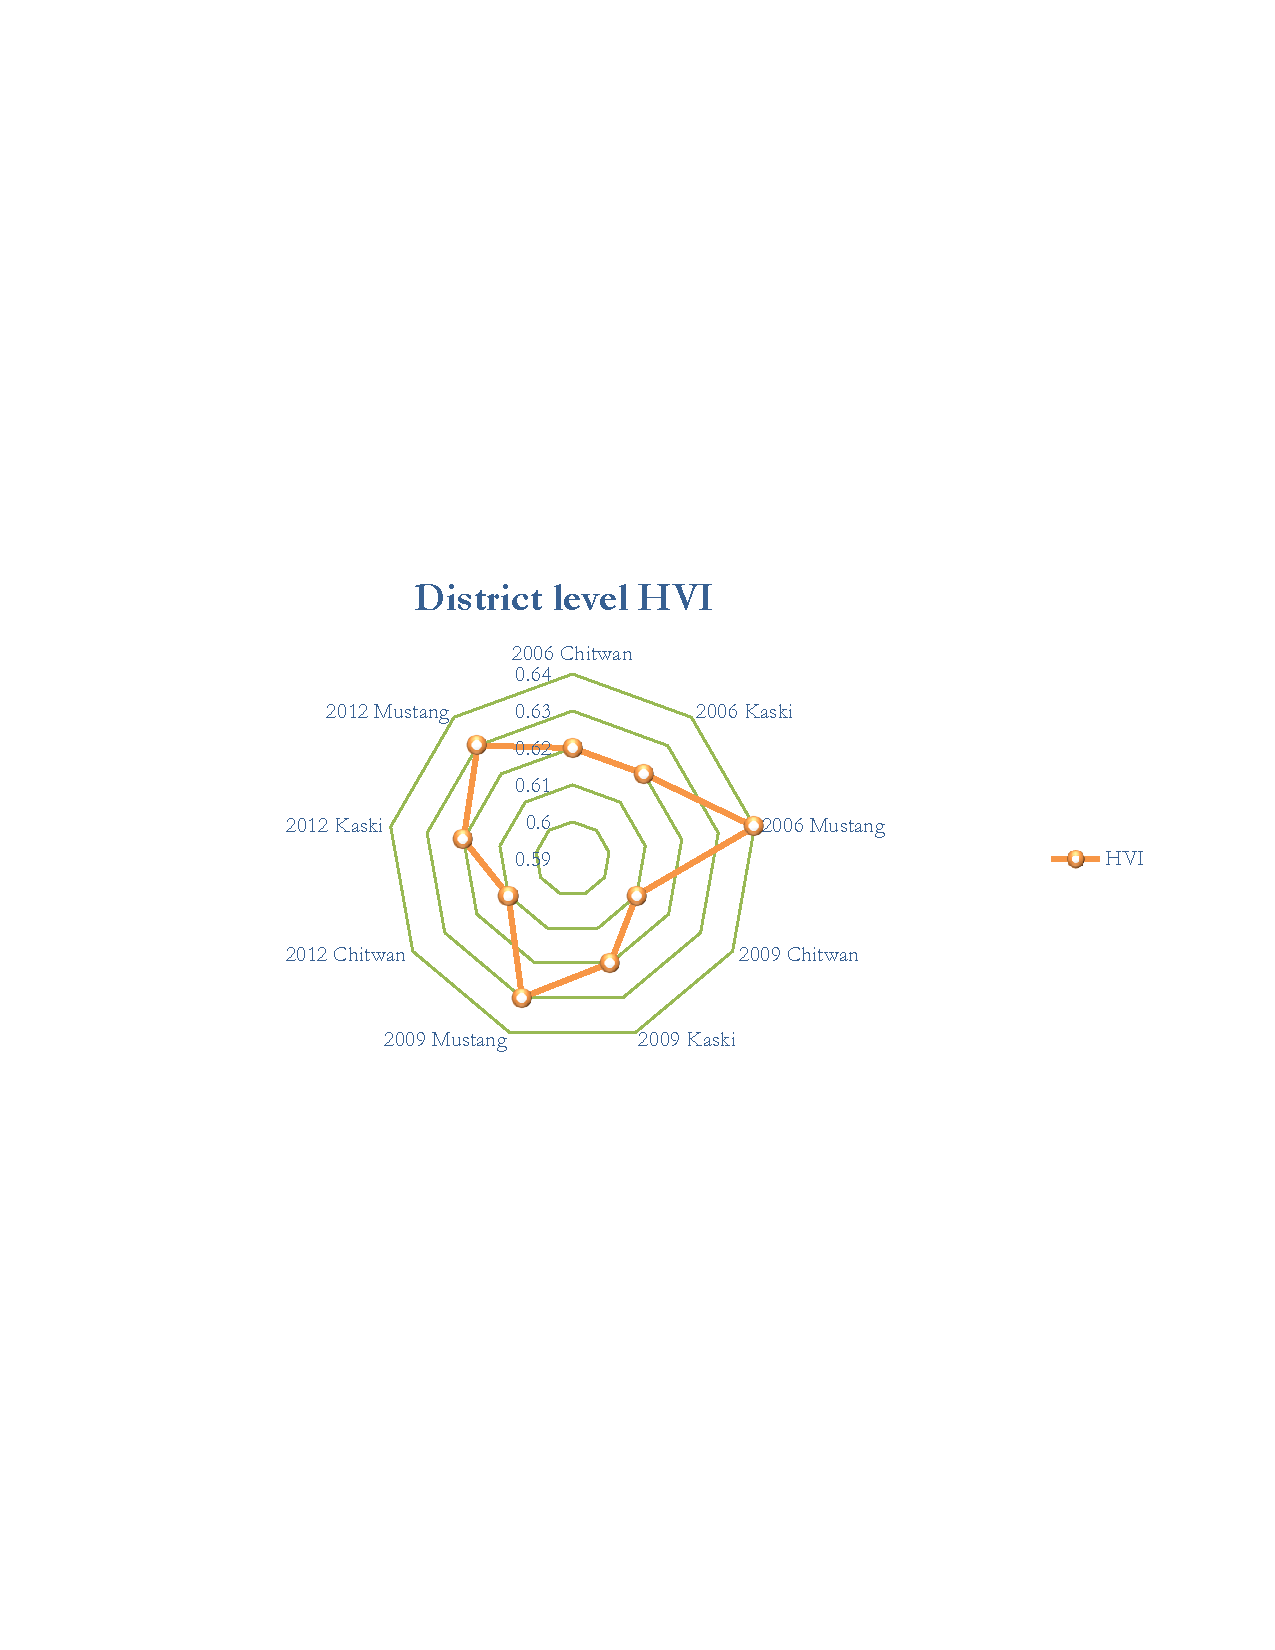
\includegraphics[scale=0.8]{./figure/HVI_Summary_District_Panel.pdf}
	\vspace{-20pt}
	\caption{District level HVI for all waves} 
	\label{fig:distictlevelhvi}
\end{figure}

Table \ref{tab:VDCmeansdhvi} represents household vulnerability Index (HVI) values for different Village Development Committees (VDC) across three districts (Chitwan, Kaski and MUstang) for three distinct years: 2006, 2009, and 2012. The VDCs within each district are Chainpur, Hemja, Kunjo, and Lete. The HVI values are provided for each combination of VDC and year.

\begin{table}[htb]
	\caption{ Village level mean and SD HVI for all waves}
	\label{vdclevelhvi}
	\resizebox{\textwidth}{!}{%
		\begin{tabular}{cccclccclcccl} \hline
			\multirow{2}{*}{\textbf{\begin{tabular}[c]{@{}c@{}}Year/\\ District\end{tabular}}} & \multicolumn{4}{c}{\textbf{2006}}                                                                                                                                                                                             & \multicolumn{4}{c}{\textbf{2009}}                                                                                                                                                                                             & \multicolumn{4}{c}{\textbf{2012}}                                                                                                                                                                                             \\ \hline
			& \textbf{Chainpur}                                     & \textbf{Hemja}                                        & \textbf{Kunjo}                                        & \textbf{Lete}                                         & \textbf{Chainpur}                                     & \textbf{Hemja}                                        & \textbf{Kunjo}                                        & \textbf{Lete}                                         & \textbf{Chainpur}                                     & \textbf{Hemja}                                        & \textbf{Kunjo}                                        & \textbf{Lete}                                         \\ \hline
			\textbf{HVI}                                                                       & \begin{tabular}[c]{@{}c@{}}0.62\\ (0.05)\end{tabular} & \begin{tabular}[c]{@{}c@{}}0.62\\ (0.04)\end{tabular} & \begin{tabular}[c]{@{}c@{}}0.65\\ (0.04)\end{tabular} & \begin{tabular}[c]{@{}l@{}}0.63\\ (0.05)\end{tabular} & \begin{tabular}[c]{@{}c@{}}0.61\\ (0.05)\end{tabular} & \begin{tabular}[c]{@{}c@{}}0.62\\ (0.04)\end{tabular} & \begin{tabular}[c]{@{}c@{}}0.64\\ (0.04)\end{tabular} & \begin{tabular}[c]{@{}l@{}}0.63\\ (0.05)\end{tabular} & \begin{tabular}[c]{@{}c@{}}0.61\\ (0.05)\end{tabular} & \begin{tabular}[c]{@{}c@{}}0.62\\ (0.05)\end{tabular} & \begin{tabular}[c]{@{}c@{}}0.64\\ (0.05)\end{tabular} & \begin{tabular}[c]{@{}l@{}}0.62\\ (0.05)\end{tabular} \\ \hline \hline
		\end{tabular}
	}
	{\textit{\ \ \ \ Note: Standard deviation in the parenthesis \\ [-1ex] \ \ \ \ \ \ \ \ Source: Author's Calculation}}
	\label{tab:VDCmeansdhvi}
\end{table}

In 2006, the mean HVI in Chainpur, Hemja, Kunjo and Lete were 0.61, 0.62, 0.65 and 0.64, respectively. Similarly, in 2009, the mean HVI for the mentioned VDCs were 0.61, 0.61, 0.64 and 0.63. The trend continued in 2012, with mean HVI of 0.61, 0.62, 0.63 and 0.61 for the above-mentioned VDCs respectively.\par 

We present the radar chart for the Village level mean HVI for all the VDCs across the survey years.\par 

The radar chart for Chainpur shows a polygon with points relatively close to each other, suggesting a stable pattern in HVI across the years. The HVI for Chainpur was 0.62 in the first wave of the survey. The HVI then declined to 0.61 and has remained stable across the second and third waves of survey. Similarly, Hemja's radar chart exhibit a relatively stable HVI across all waves of survey. The HVI has remained at 0.62 across all the waves of survey.\par 

\begin{center}
	\begin{figure}[htb]
		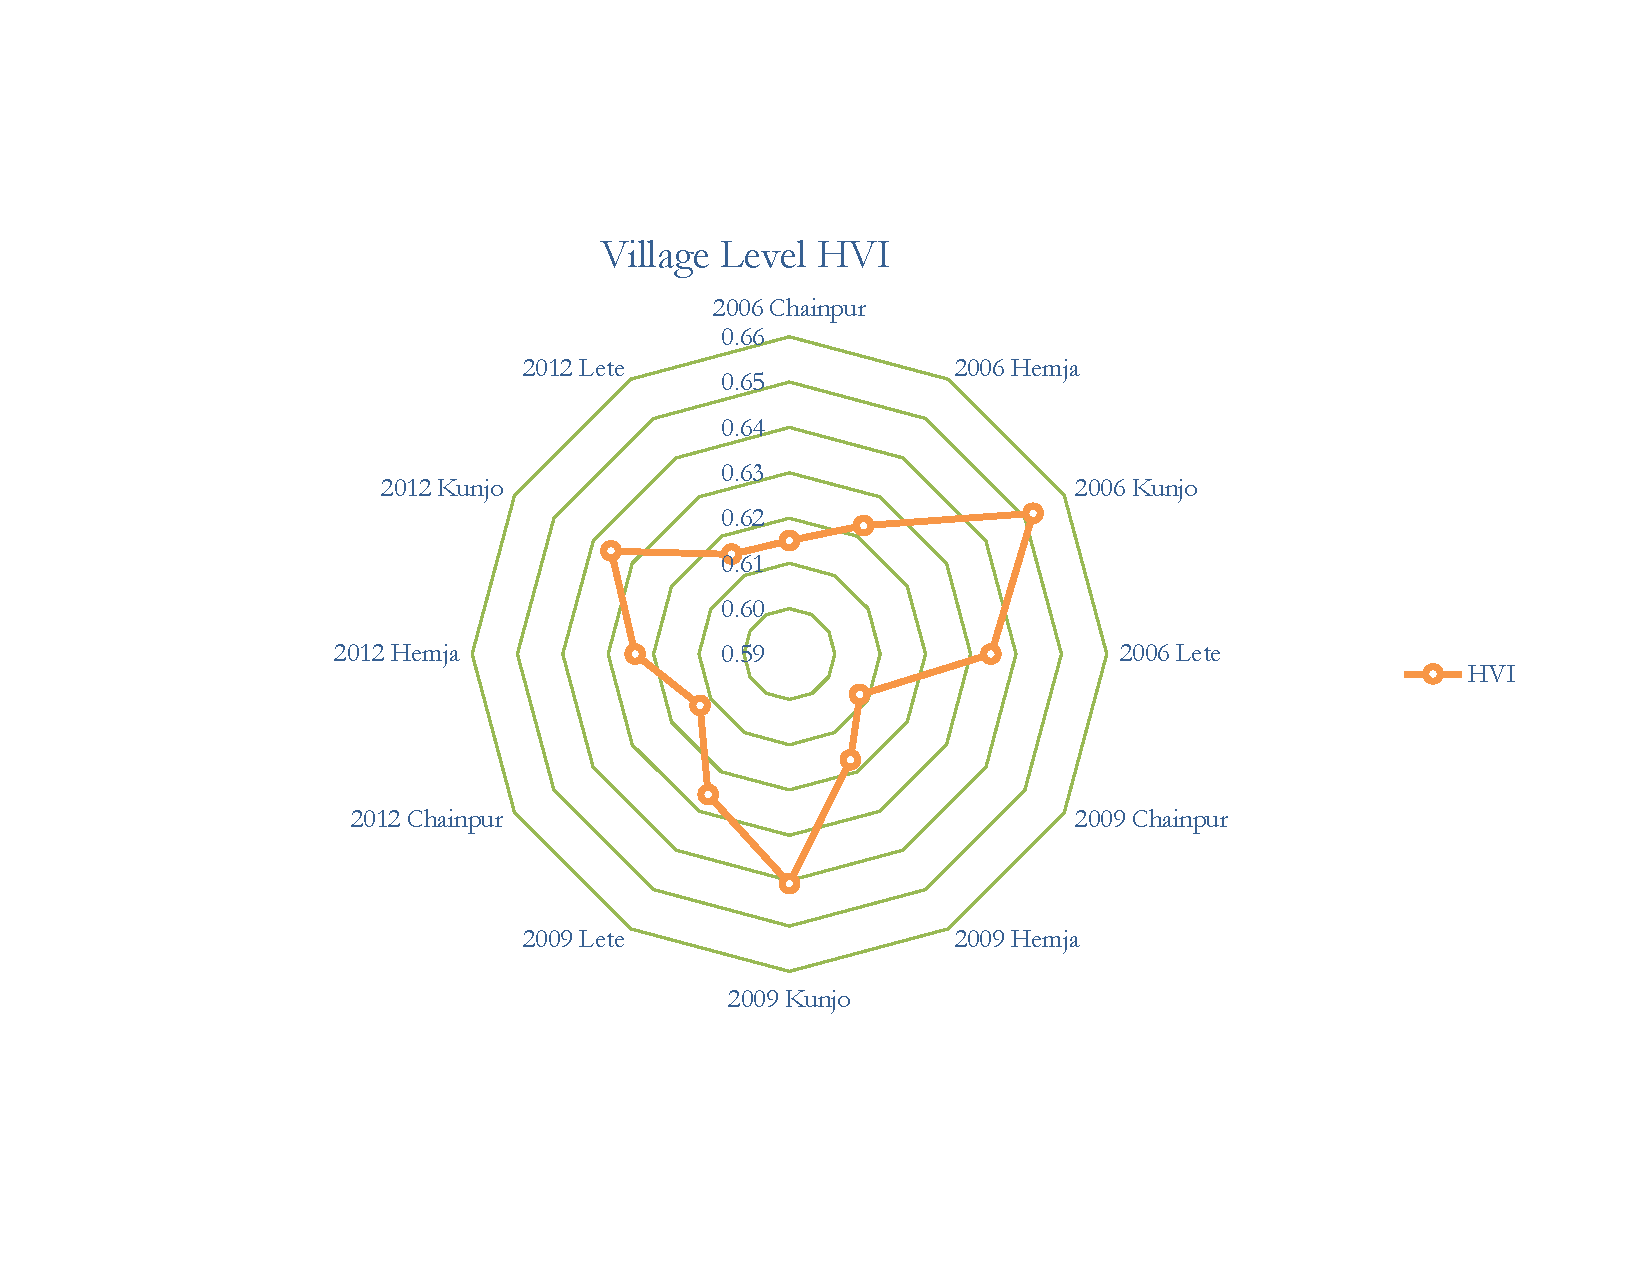
\includegraphics[scale=0.62]{figure/HVI_Summary_VDC.pdf}
		\vspace{-1.5cm}
		\caption{: Village level HVI for all waves} 
		\label{fig:vdchvisummary}
		\setlength{\belowcaptionskip}{6pt}
	\end{figure}
\end{center}

Kunjo was the highest vulnerable VDC among all the VDC. Lete followed it in terms of the vulnerability. Kunjo formed a mildly varying polygon. The HVI declined by 0.01 in 2009 from 2006. Then the HVI remains stable at 0.64 from year 2009 to 2012. The VDC had 0.65, 0.64 and 0.64 HVI in the year 2006, 2009 and 2012 respectively. This steady variation has formed a slightly fluctuating polygon.  Lete's HVI was 0.63 in the 2006 which remained consistent in the year 2009. However, it declined to 0.62 in the year 2012.   

\subsection{Component of the Household Vulnerability}
\subsubsection{Chainpur VDC, Chitwan}
Table \ref{tab:hvicomponentforchainpur} represents Chainpur VDC data for different years (2006, 2009, 2012) and various components of vulnerability, categorized into five types of capital: Human Capital (C1), Physical Capital (C2), Social Capital (C3), Livelihoods (C4), and Financial Capital (C5). The variables used in each component is in the Table 3.1. The value for the capital has been derived from equation 3.7.

\begin{center}
	\begin{table}[htb]
		\caption{Mean of the HVI components for Chainpur VDC, Chitwan}
		\label{tab:hvicomponentforchainpur}
		\resizebox{1\textwidth}{!}{%
			\begin{tabular}{ccccccc} \hline
				\textbf{Year} & \textbf{\begin{tabular}[c]{@{}c@{}}Human Capital\\  (C1)\end{tabular}} &  \textbf{\begin{tabular}[c]{@{}c@{}}Physical Capital \\ (C2)\end{tabular}} & \textbf{\begin{tabular}[c]{@{}c@{}}Social Capital \\ (C3)\end{tabular}} & \textbf{\begin{tabular}[c]{@{}c@{}}Livelihoods \\ (C4)\end{tabular}} & \textbf{\begin{tabular}[c]{@{}c@{}}Financial Capital \\ (C5)\end{tabular}} \\ \hline
				\textbf{2006} & 0.63                                                                      &  0.98                                                                         & 0.68                                                                       & 0.31                                                                 & 0.99                                                                          \\
				\textbf{2009} & 0.60                                                                                                                                                     & 0.98                                                                         & 0.72                                                                       & 0.30                                                                 & 0.99                                                                          \\
				\textbf{2012} & 0.60                                                                                                                                                     & 0.97                                                                         & 0.63                                                                       & 0.34                                                                 & 0.98   \\ \hline \hline                                                                     
			\end{tabular}
		}
		\textit{Source: Author's Calculation}
	\end{table}
\end{center}

Fig \ref{fig:hvichainpurComponent} exhibits how each component has contributed to the vulnerability level of the households in Chainpur, Chitwan. Having higher Human capital reduces vulnerability. Human Capital is exhibited to have slight decrease from 0.63 in 2006 to 0.60 in 2009 and 2012 in Chainpur. This implies that the decline in the Human capital had a negative effect on household vulnerable. Physical capital remained relatively stable around 0.98 across all rounds of survey years, suggesting a consistent level of vulnerability related to physical assets. Social Capital is demonstrated to have some variation, increasing from 0.68 in 2006 to 0.72 in 2009 and then decline to 0.63 in the year 2012. This suggests that this variation could potentially have some effect on the overall vulnerability of the household. In the livelihood component, depicts a slight dip to 0.30 in the year 2009 fro 0.31 in the year 2006. However, livelihood component have increased to 0.34 in the year 2012. Financial capital have remained stable at around 0.99 across 2006 and 2009 and only slightly decreasing to 0.98 in the year 2012.

\begin{center}
	\begin{figure}[htb]
		\vspace{-140pt}
		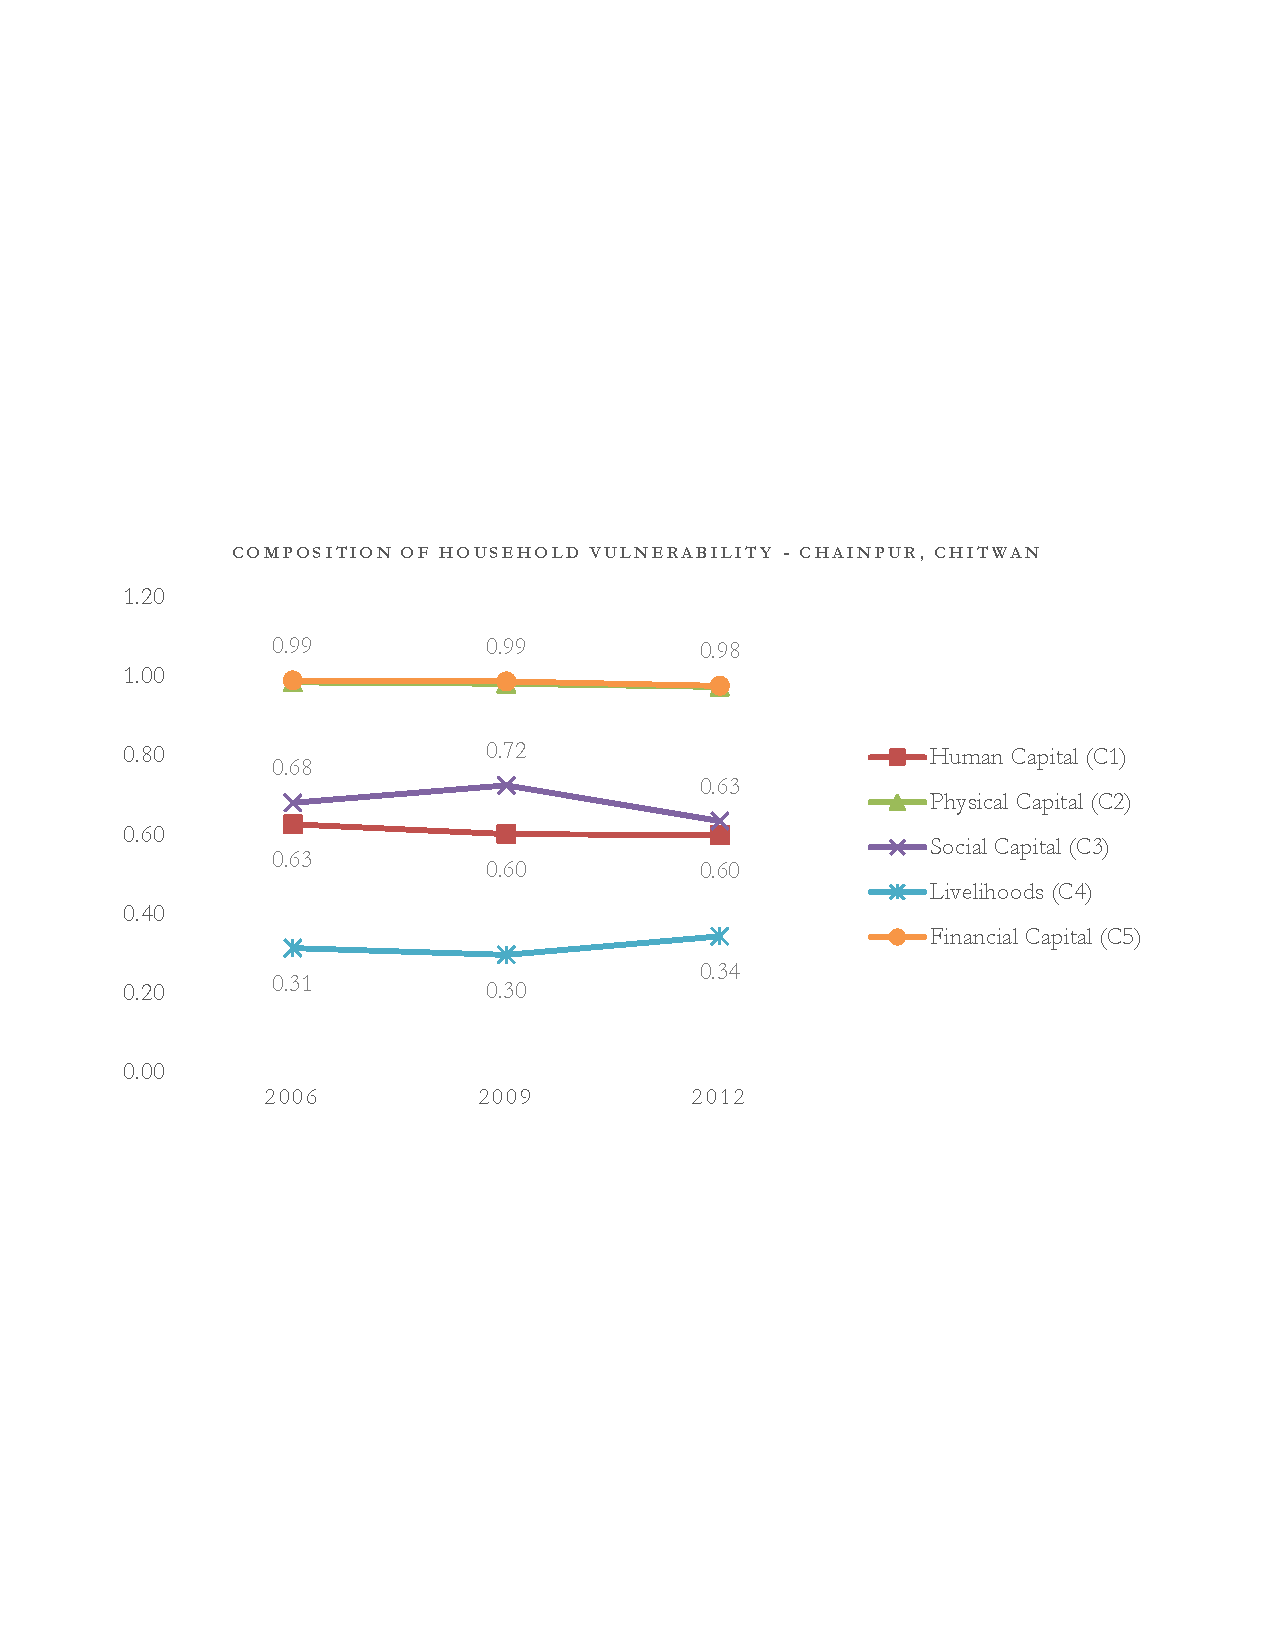
\includegraphics[scale=0.7]{figure/HVI_Component_Chainpur_line.pdf}
		\vspace{-160pt}
		\caption{Component of HVI - Chainpur VDC, Chitwan}
		\setlength{\abovecaptionskip}{6pt}
		\setlength{\belowcaptionskip}{3pt}
		\label{fig:hvichainpurComponent}
	\end{figure}
\end{center}
\vspace{-25pt}

\subsubsection{Hemja VDC, Kaski}
Table \ref{tab:hvicomponenthemja} represents data for Hemja Village Development Committee (VDC) in Kaski district across the years 2006, 2009, and 2012.\par 
\begin{table}[ht]
	\caption{Mean of the HVI components for Hemja VDC, Kaski}
	\resizebox{1\textwidth}{!}{%
		\begin{tabular}{ccccccc} \hline
			\textbf{Year} & \textbf{\begin{tabular}[c]{@{}c@{}}Human Capital\\  (C1)\end{tabular}} &  \textbf{\begin{tabular}[c]{@{}c@{}}Physical Capital \\ (C2)\end{tabular}} & \textbf{\begin{tabular}[c]{@{}c@{}}Social Capital \\ (C3)\end{tabular}} & \textbf{\begin{tabular}[c]{@{}c@{}}Livelihoods \\ (C4)\end{tabular}} & \textbf{\begin{tabular}[c]{@{}c@{}}Financial Capital \\ (C5)\end{tabular}} \\ \hline
			\textbf{2006} & 0.53                                                                      &  0.98                                                                         & 0.84                                                                       & 0.33                                                                 & 0.99                                                                          \\
			\textbf{2009} & 0.52                                                                      &  0.97                                                                         & 0.87                                                                       & 0.32                                                                 & 0.98                                                                          \\
			\textbf{2012} & 0.49                                                                                                                                                     & 0.95                                                                         & 0.62                                                                       & 0.32                                                                 & 0.96 \\      \hline  \hline                                                                \end{tabular}
	}
	\textit{Source: Author's calculation}
	\label{tab:hvicomponenthemja}
\end{table}

Figure \ref{fig:hvihemjacomponent} shows the representation of different components of vulnerability. Human Capital decreases steadily from 0.53 in 2006 to 0.52 in 2009 and further to 0.49 in 2012 in Hemja VDC over the specified years. Physical capital is exhibited a gradual decrease from 0.98 in 2006 to 0.97 in 2009 to 0.95 in 2012. Social capital also have experienced an increase from 0.84 in 2006 to 0.87 in 2009 and declined to 0.62 in 2012.Livelihoods Remains relatively stable, ranging from 0.32 to 0.33 across the three years. Financial Capital also remained relatively stable with a slight decrease from 0.99 in 2006 to 0.96 in 2012. 

Hemja VDC in Kaski district exhibits a vulnerability profile characterized by a decline in human and physical capital over the years. Social capital shows variability, with a decline from 2006 to 2012. Livelihoods and financial capital remain relatively stable. 
\begin{figure}[ht]
	\vspace{-50pt}
	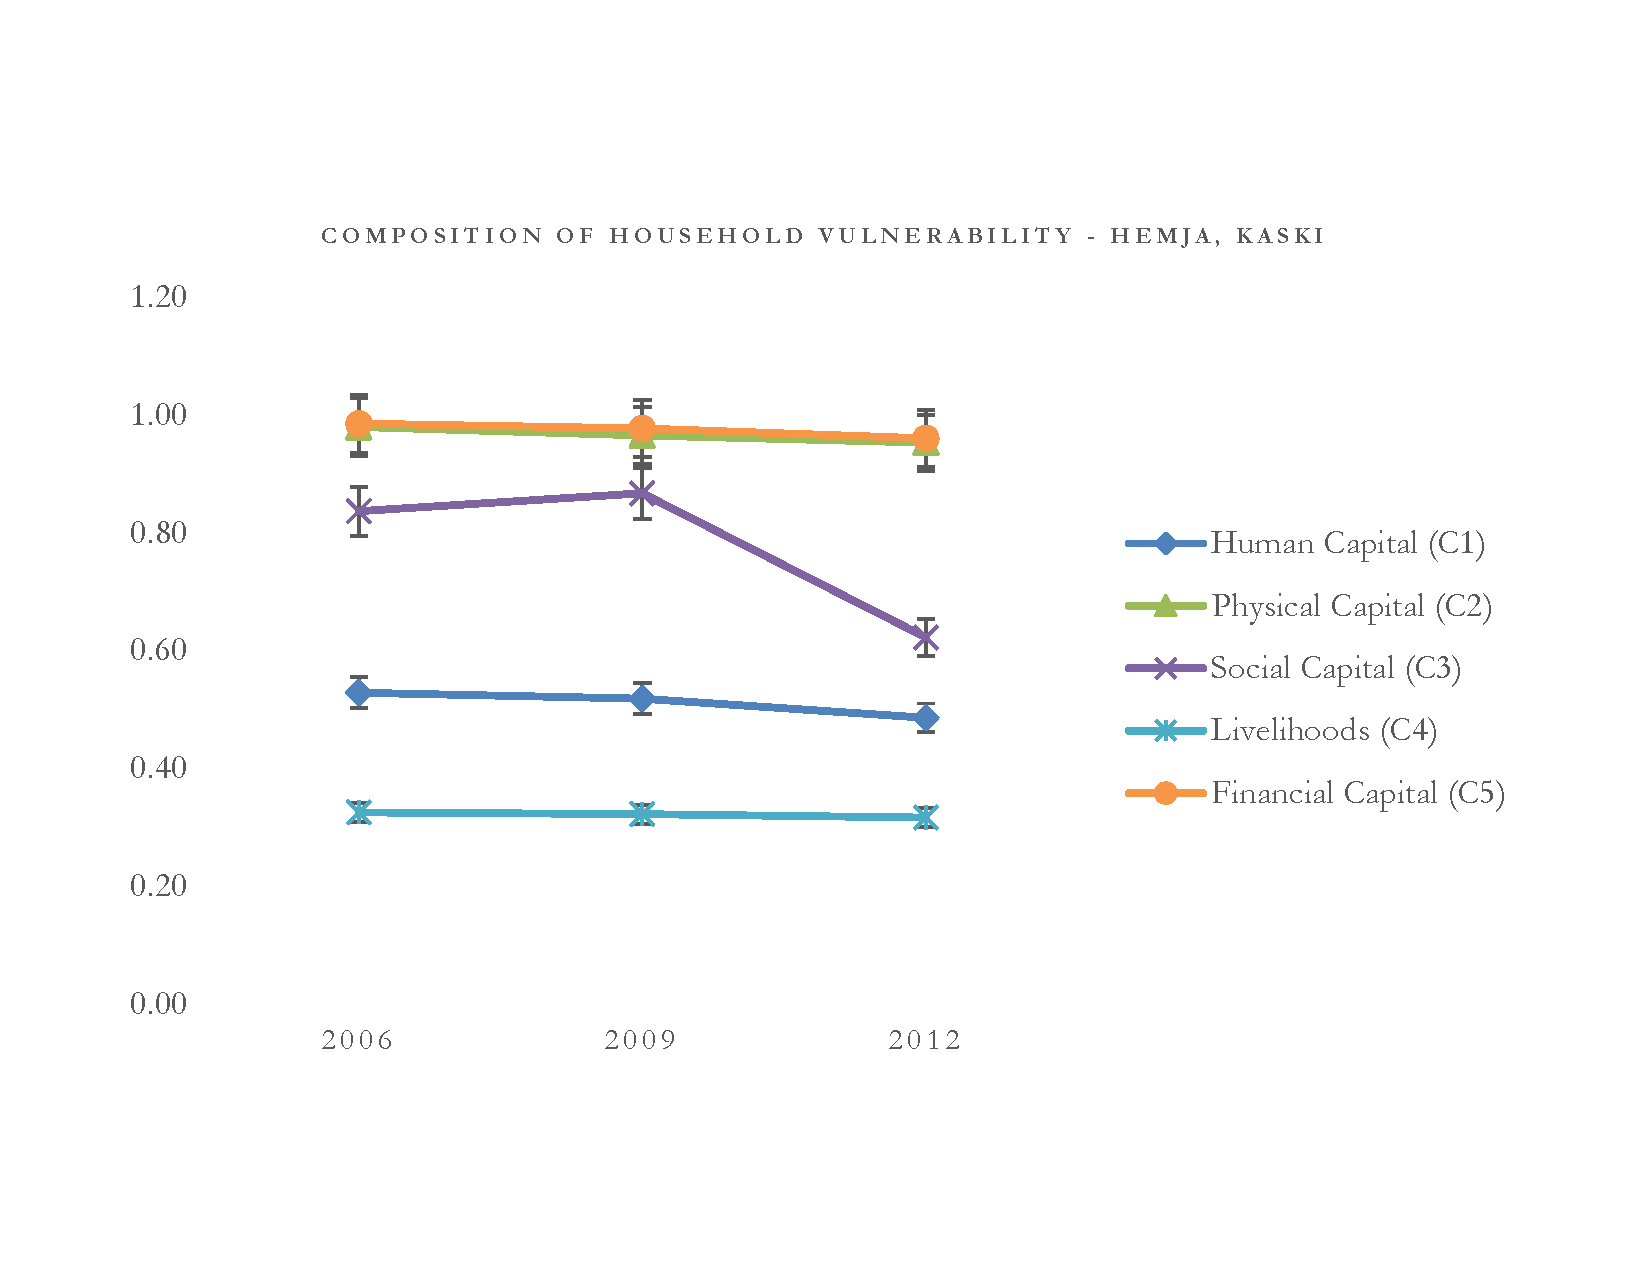
\includegraphics[scale=0.6]{figure/HVI_Component_Hemja_line.pdf}
	\vspace{-50pt} % reduce the gap below the figure before caption
	\caption{Component of HVI - Hemja VDC, Kaski}
	\setlength{\abovecaptionskip}{4pt}
	\label{fig:hvihemjacomponent}
\end{figure}

\subsubsection{Kunjo VDC, Mustang}
Table \ref{tab:hvikunjocomponents} represents data for Kunjo Village Development Committee (VDC) in Mustang district across the years 2006, 2009, and 2012. Each row corresponds to a specific year, and the columns represent different components of vulnerability.
\begin{table}[ht]
	\caption{Mean of the HVI components for Kunjo VDC, Mustang}
	\resizebox{1\textwidth}{!}{%
		\begin{tabular}{ccccccc} \hline
			\textbf{Year} & \textbf{\begin{tabular}[c]{@{}c@{}}Human Capital\\  (C1)\end{tabular}} &  \textbf{\begin{tabular}[c]{@{}c@{}}Physical Capital \\ (C2)\end{tabular}} & \textbf{\begin{tabular}[c]{@{}c@{}}Social Capital \\ (C3)\end{tabular}} & \textbf{\begin{tabular}[c]{@{}c@{}}Livelihoods \\ (C4)\end{tabular}} & \textbf{\begin{tabular}[c]{@{}c@{}}Financial Capital \\ (C5)\end{tabular}} \\ \hline
			\textbf{2006} & 0.65                                                                      &  0.97                                                                         & 0.59                                                                       & 0.31                                                                 & 0.97                                                                          \\
			\textbf{2009} & 0.63                                                                      &  0.97                                                                         & 0.63                                                                       & 0.24                                                                 & 0.97                                                                          \\
			\textbf{2012} & 0.64                                                                      &  0.97                                                                         & 0.82                                                                       & 0.32                                                                 & 0.96  \\ \hline \hline                                                                      
		\end{tabular} 
	}		
	\textit{Source: Author's calculation}
	\label{tab:hvikunjocomponents}
\end{table}

Human capital component was 0.65 in 2006, decreases to 0.63 in 2009, and slightly increases to 0.64 in 2012. Physical capital remains constant at 0.97 across all three years. Social capital component 0.59 in 2006, increases to 0.63 in 2009, and further increases to 0.82 in 2012. Livelihood components exhibits variability across the years. The average value decreased to 0.24 in 2009 from 0.31 in 2006 and then increasing to 0.32 in 2012. Financial capital remained relatively stable at around 0.97 across three years.\par  

Overall, Human capital and financial capital exhibited slight fluctuations. Physical capital remained stable. Social capital experienced a significant increase. Livelihood show variability with a dip in 2009 and subsequent increase in 2012.\par      	
\begin{figure}[htb]
	\vspace{-40pt}
	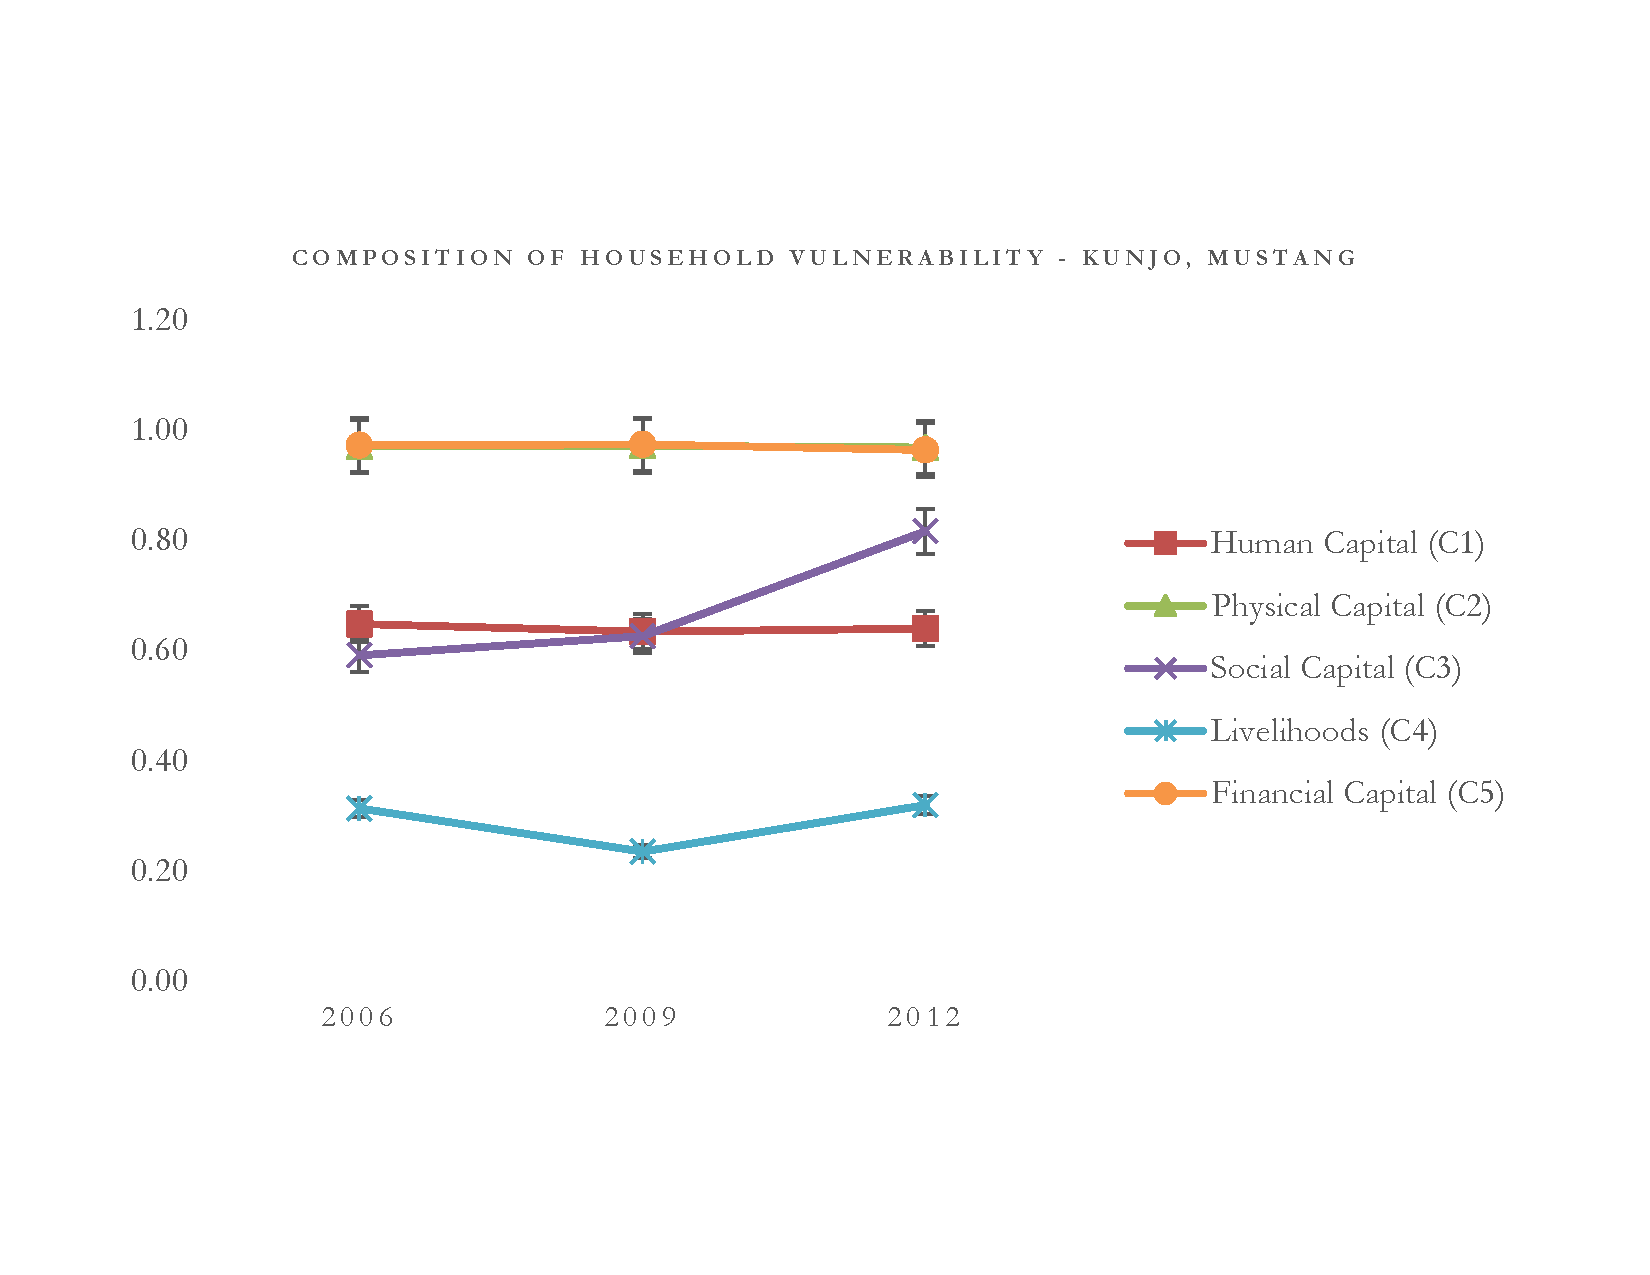
\includegraphics[scale=0.6]{figure/HVI_Component_Kunjo_line.pdf}
	\vspace{-50pt}
	\caption{ Component of HVI - Kunjo VDC, Mustang}
	\setlength{\abovecaptionskip}{4pt}
	\label{fig:hvikunjocomponents}
\end{figure}

\subsubsection{Lete VDC, Mustang}
The table represents data for Lete Village Development Committee (VDC) in Mustang district across the years 2006, 2009, and 2012. Each row corresponds to a specific year, and the columns represent different components of vulnerability.
\begin{table}[htb]
	\caption{Mean of the HVI components for Lete VDC, Mustang}
	\resizebox{1\textwidth}{!}{%
		\begin{tabular}{ccccccc} 
			\hline
			\textbf{Year} & \textbf{\begin{tabular}[c]{@{}c@{}}Human Capital\\  (C1)\end{tabular}} &  \textbf{\begin{tabular}[c]{@{}c@{}}Physical Capital \\ (C2)\end{tabular}} & \textbf{\begin{tabular}[c]{@{}c@{}}Social Capital \\ (C3)\end{tabular}} & \textbf{\begin{tabular}[c]{@{}c@{}}Livelihoods \\ (C4)\end{tabular}} & \textbf{\begin{tabular}[c]{@{}c@{}}Financial Capital \\ (C5)\end{tabular}} \\ \hline
			\textbf{2006} & 0.61                                                                      &  0.96                                                                         & 0.66                                                                       & 0.38                                                                 & 0.96                                                                          \\	\textbf{2009} & 0.61                                                                      &  0.97                                                                         & 0.69                                                                       & 0.31                                                                 & 0.96                                                                          \\ \textbf{2012} & 0.59                                                                      &  0.97                                                                         & 0.70                                                                       & 0.36                                                                 & 0.94 \\ \hline  \hline                                                            		\end{tabular} 
	}
	\textit{Source: Author's calculation}
	\label{tab:hviletecomponents}
\end{table}

Human Capital indicates stability with a minor decline in. The human capital component was 0.61 in 2006, remains constant in the following year, and slightly decreases to 0.59 in the year 2012. Physical Capital suggests stability and a slight improvement. The physical capital increases from 0.96 in 2006 to 0.97 in the year 2009 and remains constant in 2012. Social Capital is exhibited to have consistent rise across the years. It was 0.66 in the year 2006, increases to 0.69 in the year 2009, and further increases to 0.70 in the year 2012. Livelihoods component is fluctuating across the years. Livelihood decrease from 0.38 in 2006 to 0.31 in 2009, and then increasing to 0.36 in 2012. Financial capital indicates generally stable but slightly declining level of vulnerability related to financial resources. Financial Capital component was 0.96 in 2006, remained constant in 2009, and decreased slightly to 0.94 in 2012.\par  

We could observe stability in physical capital and social capital with minor fluctuations. human capital and financial capital exhibited a minor decline. Livelihood showed variability with a dip in one wave and increase in another wave.\par  

\begin{figure}[htb]
	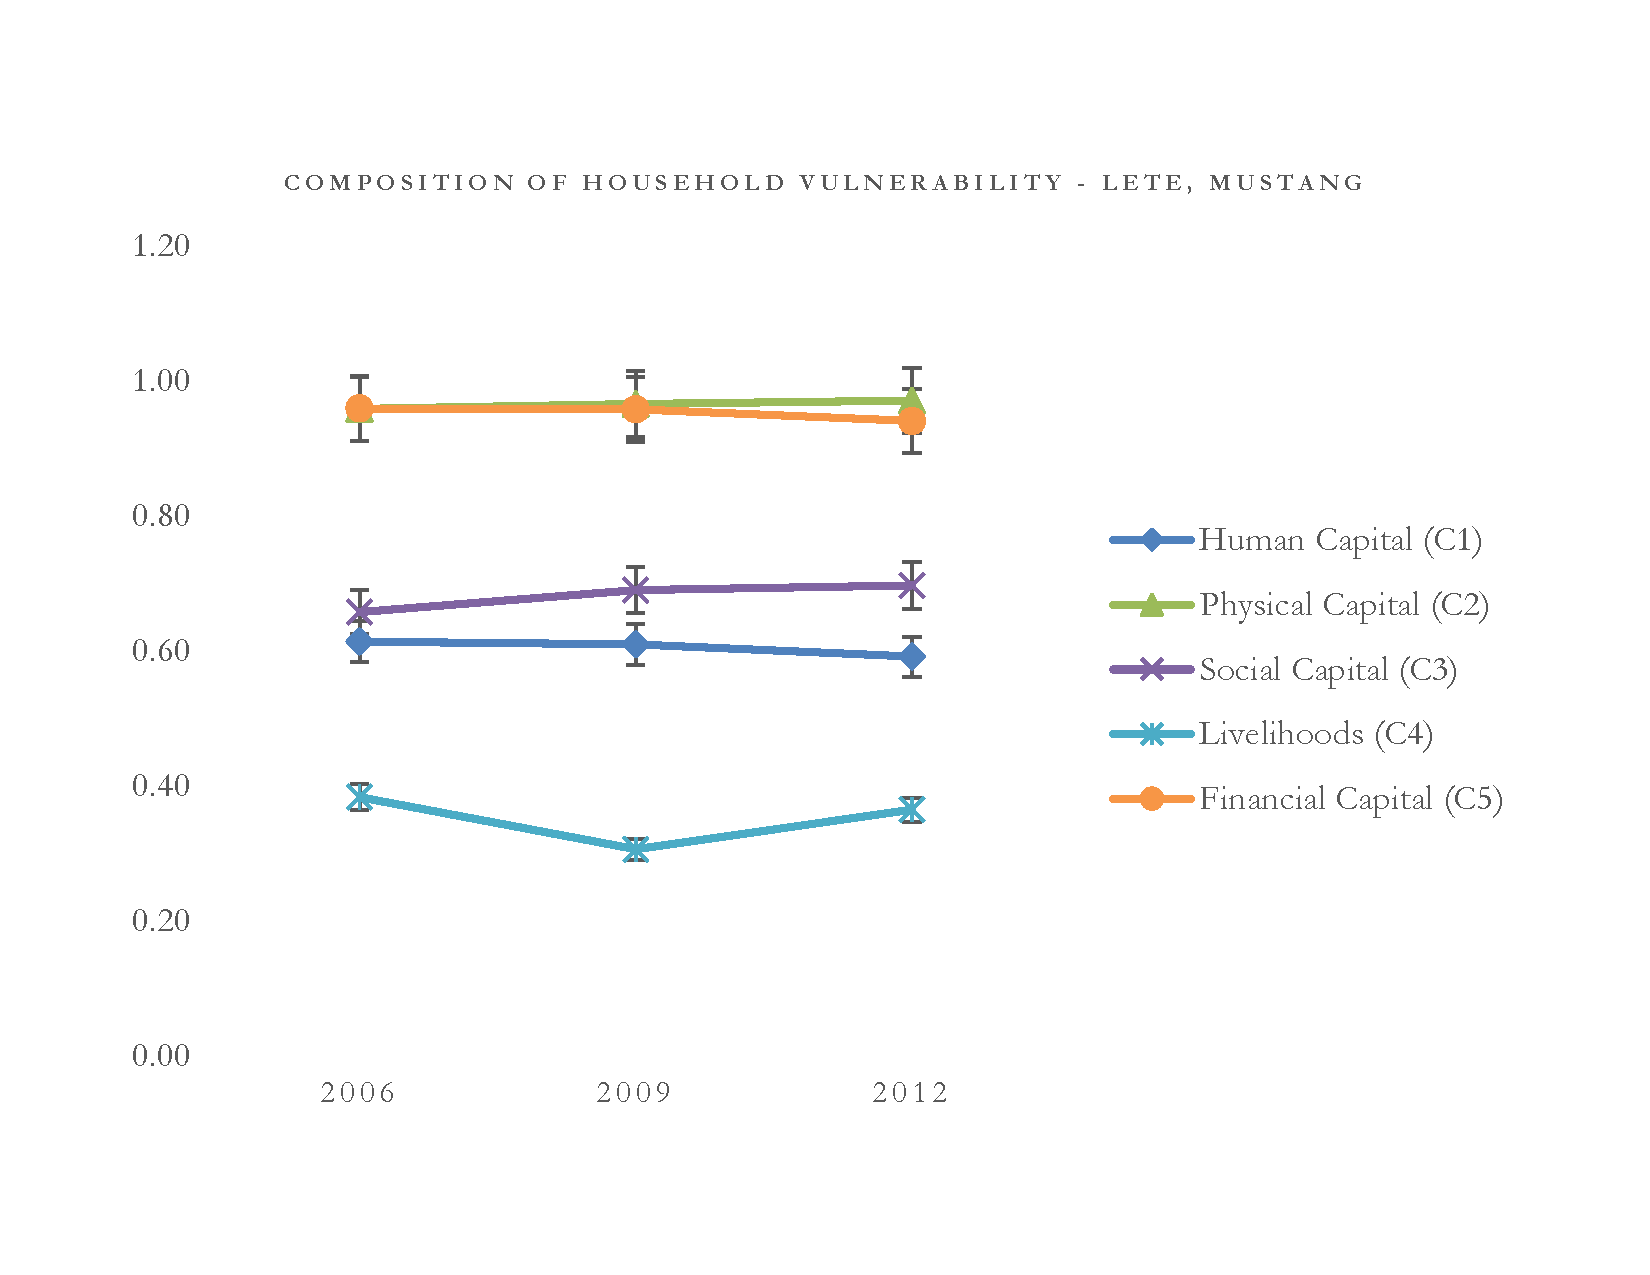
\includegraphics[scale=0.6]{figure/HVI_Component_Lete_line.pdf}
	\caption{Component of HVI - Lete VDC, Mustang}
	\setlength{\abovecaptionskip}{1pt}
	\label{fig:hviletecomponents}
\end{figure}

A panel summary of the components of the HVI is presented in Appendix Table 2. Further a composed stacked line with markers is presented in Appendix Fig 1.

\subsection{Persistence and Transience of Household Vulnerability}
Figure \ref{fig:sankey} is a Sankey diagram presenting the persistence and transitions of the household vulnerability level across the waves of survey. The value labels represent the number of households that are in the corresponding vulnerability.\par 
\begin{figure}[htb]
	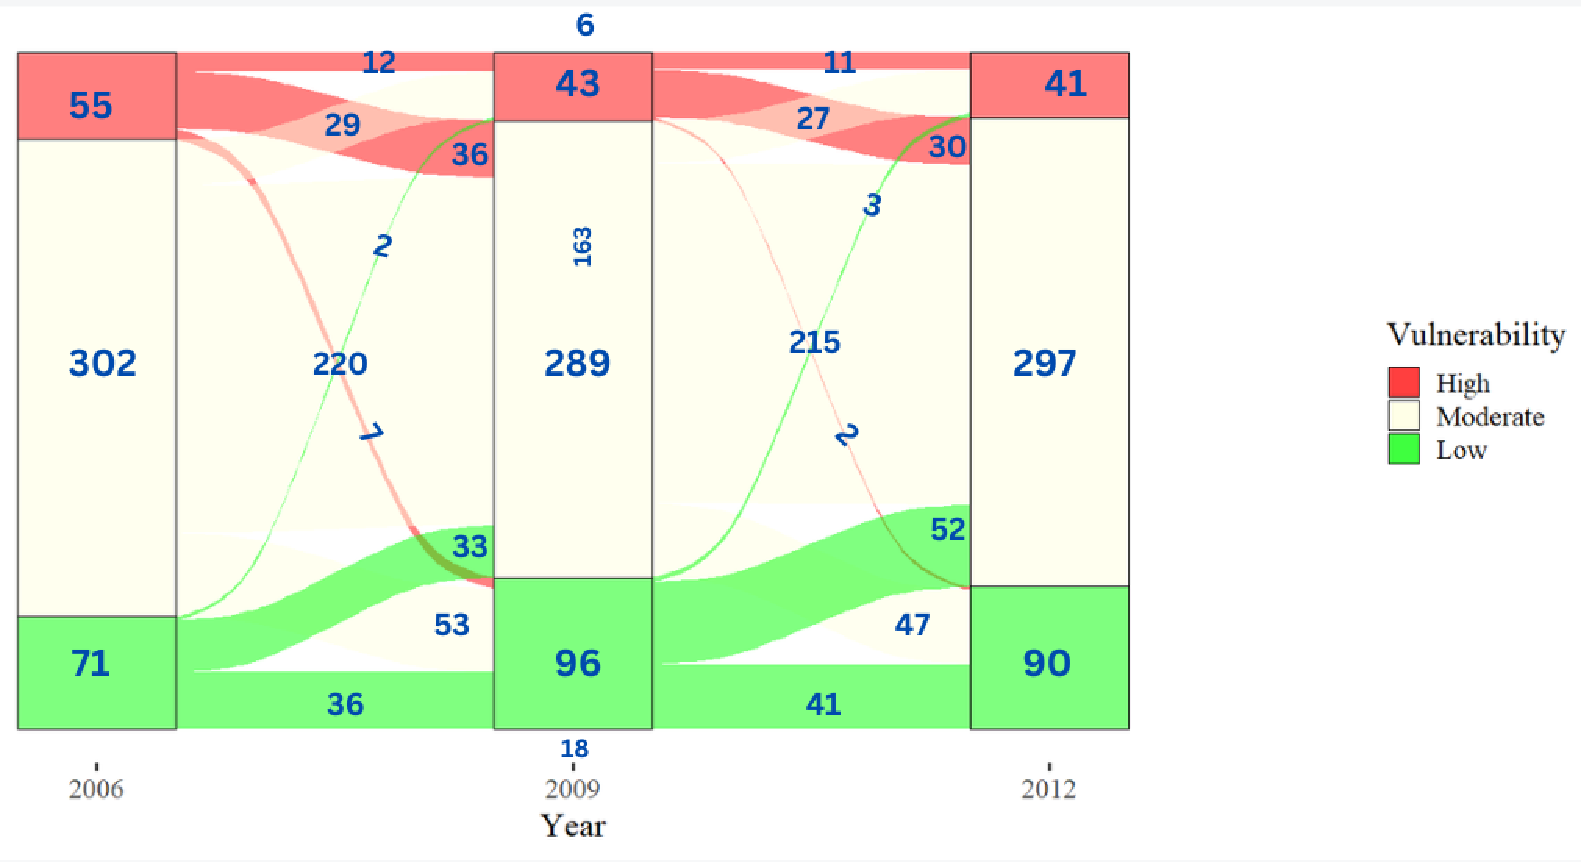
\includegraphics[scale=0.6]{./figure/Sankey}
	\caption{Persistence and Transience of Household Vulnerability}
	\setlength{\abovecaptionskip}{2pt}
	\label{fig:sankey}
\end{figure}

The details of the Vulnerability level across the survey waves (2006, 2009, 2012) is presented in Table 4.9. In the table, in 2006 there are 55 households categorised as "High", 302 as "Moderate" and 71 as "Low" vulnerability level. In 2009, the number of households classified as "High" vulnerability decreased to 43, "Moderate" vulnerability decreased to 289, and "Low" vulnerability increased to 96. In 2012, the number of households classified as "High" vulnerability further decreased to 41, "Moderate" vulnerability increased slightly to 297, and "Low" vulnerability decreased to 90.\par 

\begin{table}[htb]
	%\captionsetup{labelformat=empty}
	%\captionsetup{labelformat=empty, skip=-7pt} % Adjust the skip to reduce space
	\caption{{Vulnerability level across the waves of survey}
		\begin{center}
		\begin{tabular}{lccc} \hline
			\textbf{Vulnerability level} & \textbf{2006}            & \textbf{2009}            & \textbf{2012}           \\ \hline
			High                         & 55                       & 43                       & 41                      \\
			Moderate                     & 302                      & 289                      & 297                     \\
			Low                          & 71                       & 96                       & 90                \\ \hline \hline     
		\end{tabular}\\
	\end{center}\vspace{-8pt}
	\textit{\ \ \ \ \ \ \ \ \ \ \ \ \ \ \  \ \ \ \ \ \ \ \ Source:Author's calculation}
	\label{tab:Vulnerabilitylevels}
\end{table}

Table 4.10 presents the transition of the vulnerability levels of the households. This table shows the household transitioning from one vulnerability level to another between each pair of survey years. For example, from 2006 to 2009, there were 12 households that were "High" vulnerability in 2006 and remained "High" vulnerability in 2009. Similarly, there were 36 households that were "High" vulnerability in 2006 and transitioned to "Moderate" vulnerability in 2009.

\begin{table}[H]
	\captionsetup{labelformat=empty}
	\captionsetup{labelformat=empty, skip=-7pt} % Adjust the skip to reduce space
	\caption{{Table 4.10}: Transition matrix of the household vulnerability}
	\label{tab:Vulnerabilitytransitions}	\begin{center}
		\begin{tabular}{lcc} \hline
			\textbf{Vulnerability Level} & \textbf{2006-2009} & \textbf{2009-2012} \\ \hline
			High to High                 & 12                 & 11                 \\
			High to low                  & 7                  & 2                  \\
			High to Moderate             & 36                 & 30                 \\
			Low to High                  & 2                  & 3                  \\
			Low to Low                   & 36                 & 41                 \\
			Low to moderate              & 33                 & 52                 \\
			Moderate to High             & 29                 & 27                 \\
			Moderate to low              & 53                 & 47                 \\
			Moderate to Moderate         & 220                & 215       \\ \hline \hline        
		\end{tabular} \\
	\end{center}\vspace{-8pt}
	\textit{\ \ \ \ \ \ \ \ \ \ \ \ \ \ \ \ \ \ \ Source:Author's calculation}
\end{table}

Table 4.11 presents the persistence of vulnerability across the survey waves. It highlights the number of households that remained in the same vulnerability level throughout the entire period of 2006 to 2012. There were 6 households that remained in the "High" vulnerability category from 2006 to 2012. Similarly, there were 18 households that remained in the "Low" vulnerability category throughout the same period.



\begin{table}[H]
	\captionsetup{labelformat=empty}
	\captionsetup{labelformat=empty, skip=-7pt} % Adjust the skip to reduce space
	\caption{{Table 4.11}: Persistence of vulnerability the household 2006-2009-2012}
	\label{tab:Vulnerabilitypersistence}
	\begin{center}
		\begin{tabular}{lc} \hline
			\textbf{Vulnerability level} & \textbf{No. of Households} \\	\hline
			High to High & 6 \\
			Low to Low            & 18         \\
			Moderate to Moderate  & 163  \\ \hline \hline     
		\end{tabular} \\
	\end{center}\vspace{-8pt}
	\textit{\ \ \ \ \ \ \ \ \ \ \ \ \ \ \ \ \ \ \ \ \ \ Source:Author's calculation}
\end{table}